%Based on the code of Yiannis Lazarides
%http://tex.stackexchange.com/questions/42602/software-requirements-specification-with-latex
%http://tex.stackexchange.com/users/963/yiannis-lazarides
%Also based on the template of Karl E. Wiegers
%http://www.se.rit.edu/~emad/teaching/slides/srs_template_sep14.pdf
%http://karlwiegers.com
\documentclass{scrreprt}
\usepackage{listings}
\usepackage{underscore}
\usepackage[margin=3.0cm]{geometry}
\usepackage{enumitem}
\usepackage{graphicx}
\usepackage[bookmarks=true]{hyperref}
\usepackage[english, spanish]{babel}
\usepackage[utf8]{inputenc}
\usepackage{float}
\usepackage{xcolor}
\usepackage{fancyhdr}
\usepackage[export]{adjustbox}

\hypersetup{
    bookmarks=false,        % show bookmarks bar?
    pdftitle={Especificación de Requerimientos de Software},    % title
    pdfauthor={},           % author
    pdfsubject={},          % subject of the document
    pdfkeywords={},         % list of keywords
    colorlinks=true,        % false: boxed links; true: colored links
    linkcolor=blue,         % color of internal links
    citecolor=black,        % color of links to bibliography
    filecolor=black,        % color of file links
    urlcolor=purple,        % color of external links
    linktoc=page            % only page is linked
}

\def\myversion{1.0.1}
\date{}
\usepackage{hyperref}
\usepackage{etoolbox}

%%%%%%%%%%%
% Configurar estilo de header y footer
\fancypagestyle{plain}{
  \fancyhf{}
  \lfoot{
\includegraphics[scale=0.08,valign=c]{images/space_logo.png}}
  \rfoot{Pág. \thepage}
}

\pagestyle{fancy}
\fancyhf{}
\lfoot{
\includegraphics[scale=0.08,valign=c]{images/space_logo.png}}
\rfoot{Pág. \thepage}

\renewcommand{\headrulewidth}{0pt} % linea de header invisible
\renewcommand{\footrulewidth}{0.4pt} % linea de footer delgada

%%%%%%%%%%

\begin{document}

\begin{flushright}
	\rule{16cm}{0.2cm}\vskip1cm
    \begin{bfseries}
        \Huge{ESPECIFICACIÓN DE REQUERIMIENTOS\\DEL SISTEMA}\\
        \vspace{0.5cm}
        para\\
        \vspace{0.5cm}
        Sistema de preprocesamiento y segmentación de células\\
        \vspace{1.0cm}
        \LARGE{Versión \myversion}\\
        \vspace{1.0cm}
        Preparado por:\\ \vspace{0.5cm}
        	José Alvarado Chaves, 201129079\\
            Reggie Barker Guillén, 2014050578\\
            Joel Barrantes Garro, 2013120962\\
            Joel Schuster Valverde, 2014096796\\                        
        \vspace{1.5cm}
        Instituto Tecnológico de Costa Rica\\
        \vspace{1.5cm}
        \today\\
    \end{bfseries}
\end{flushright}


\tableofcontents


\chapter*{Historial de revisiones}

\begin{center}
    \begin{tabular}{|c|c|c|c|}
        \hline
	    Id & Fecha & Motivo del cambio & Versión\\
        \hline
	    1 & 21/03/2017 & Redacción inicial del documento & 1.0\\
        \hline        
        2 & 26/03/2017 & Redacción final del documento & 1.0\\
        \hline
        2 & 26/04/2017 & Actualización de prioridades & 1.0.1\\
        \hline
    \end{tabular}
\end{center}

%%%%%%%%%%%%%%%%%%%%%%%%%%%%%%%%%%%%%%%%%%%%%%%%%%%%%%%%%
%%% Link al documento estandar ISO-IEC-IEEE 29148-2011 %%
%%% http://docdro.id/LvmnK4Y					       %%	 
%%%%%%%%%%%%%%%%%%%%%%%%%%%%%%%%%%%%%%%%%%%%%%%%%%%%%%%%%

\chapter{Introducción}

\section{Propósito del sistema}
El Sistema de Preprocesamiento y Análisis CElular (SPACE) tiene como propósito automatizar el análisis de una secuencia de imágenes obtenidas a partir de microscopia de fluorescencia, como parte del proceso de investigación del laboratorio de quimiosensibilidad tumoral de la Escuela de Microbiología, de la Universidad de Costa Rica. La base del sistema busca automatizar el conteo de las células en la serie de imágenes.

\section{Alcance del sistema}
Desde su inauguración en agosto de 2016, el laboratorio de quimiosensibilidad tumoral de la Universidad de Costa Rica se ha dedicado ha realizar el servicio de prueba diagnóstica ATP-TCA. El doctor Steve Quirós está a cargo del laboratorio, el cual emplea tecnología de punta, (como es el componente biocomputacional y la Biología de Sistemas) para generar conocimiento científico que ayude a avanzar hacia la terapia personalizada del cáncer.\\

\begin{figure}[H]
	\centering
    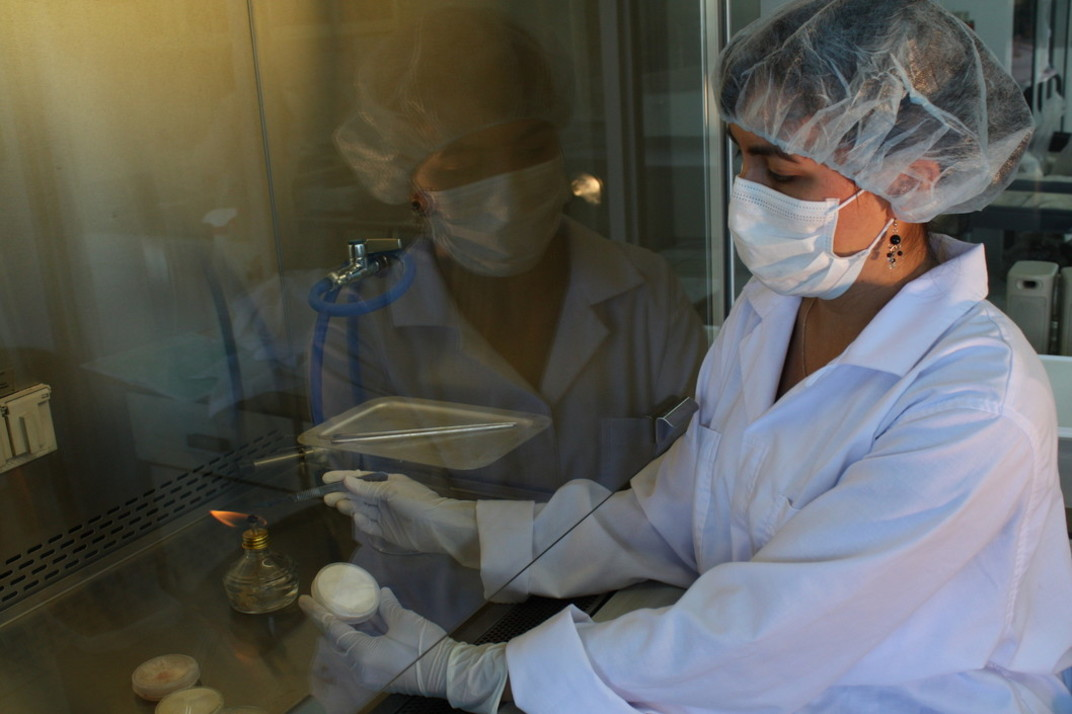
\includegraphics[width=0.8\linewidth]{images/laboratorio.jpg}
    \caption{Análisis de sangre. Imagen con fines ilustrativos.}\label{imagenLab}
\end{figure}

El sistema SPACE permitirá el preprocesamiento y análisis de características específicas de un lote de imágenes de células, fotografiadas con el equipo de microscopía del laboratorio.\\

El sistema SPACE especificado en este documento formará parte del conjunto de herramientas usadas en el proceso de la prueba diagnóstica ATP-TCA. Como parte de este conjunto, se espera que SPACE coexista con las herramientas usadas actualmente en el laboratorio de quimiosensibilidad tumoral, específicamente, con el equipo de cómputo y el microscopio multi-modal y de captura de imágenes celulares: Cytation 3.


\section{Perspectiva del sistema}

\subsection{Contexto del sistema}
En el laboratorio de quimiosensibilidad tumoral, se realizan experimentos sobre conjuntos de células para determinar su respuesta a distintos medicamentos quimioterapéuticos, y se monitorean utilizando varias técnicas para extraer información sobre cada célula, entre ellas:

\begin{enumerate}[label=\alph*.]
	\item Microscopía por fluorescencia;
    \item Citometría de flujo;
    \item Cultivo de células;
    \item Conteo celular;
    \item Y tinción histoquímica.
\end{enumerate}

El laboratorio cuenta con un equipo computacional sencillo y una serie de equipo de laboratorio para el estudio de las células, entre ellos el anteriormente mencionado microscopio multi-modal, Cytation 3. Este dispositivo capturará imágenes durante varios días para generar una muestra considerable que permita hacer mediciones acertadas sobre las células.

\begin{figure}[H]
	\centering
    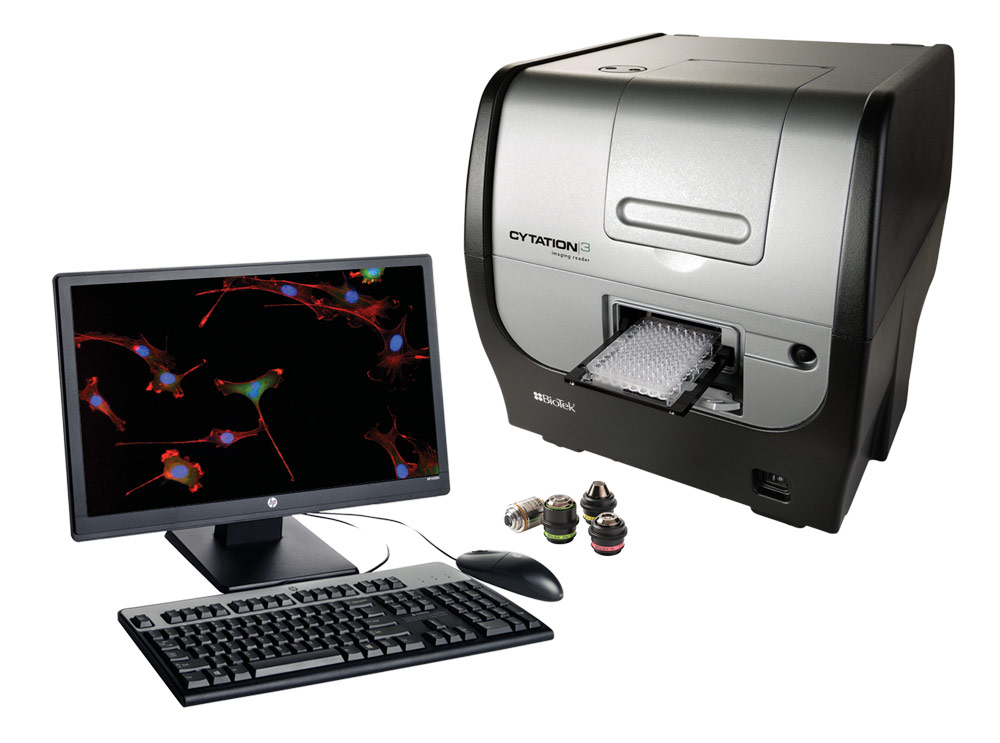
\includegraphics[width=0.7\linewidth]{images/cytation3.jpg}
    \caption{Equipo disponible en laboratorio de quimiosensibilidad tumoral.}\label{imagenCytation}
\end{figure}

El dispositivo se encuentra enlazado con una de las computadoras de usuario único del laboratorio, la cual guarda todas las fotografías de las células en su disco duro. Debido a que el equipo de computación es modesto, es preferible que el sistema SPACE sea independiente del hardware del laboratorio, además para simplificar el proceso para los investigadores. 

Como parte del nuevo sistema, el laboratorio aprovechará su conexión a Internet para subir las imágenes almacenadas en el disco duro al servidor de la solución, donde serán pre-procesadas, procesadas y se extraerá información de interés para los investigadores mediante algoritmos de visión computacional. Dicha información se almacena a su vez en el servidor, y los usuarios podrán acceder a ella mediante la web de forma sencilla.


\subsection{Funciones del sistema}

El sistema SPACE provee al usuario las siguientes funcionalidades para el análisis  de imágenes de células en tejido de glioblastoma:\\

%Documento de requerimientos
%Tabla con cada requerimiento de la forma: Identificador | Nombre de requerimiento | Descripción | Prioridad 

% SP001
\begin{tabular}{ |p{3cm}|p{10cm}|  }
  \hline
  \textbf{Identificación} & SP001  \\
  \hline
  \textbf{Nombre} & Manejo de sesiones de usuario \\
  \hline
  \textbf{Características} & El sistema debe permitir el registro, ingreso y cierre de sesiones de usuario. \\
  \hline
  \textbf{Prioridad} & Media \\
  \hline
\end{tabular}

\vspace{0.8cm}

% SP002
\begin{tabular}{ |p{3cm}|p{10cm}|  }
  \hline
  \textbf{Identificación} & SP002  \\
  \hline
  \textbf{Nombre} & Subida de imágenes \\
  \hline
  \textbf{Características} & El sistema debe permitir que el usuario suba hasta tres lotes de imágenes. \\
  \hline
  \textbf{Prioridad} & Media \\
  \hline
\end{tabular}

\vspace{0.8cm}

% SP003
\begin{tabular}{ |p{3cm}|p{10cm}|  }
  \hline
  \textbf{Identificación} & SP003  \\
  \hline
  \textbf{Nombre} & Visualización de lotes pendientes  \\
  \hline
  \textbf{Características} & El sistema debe permitir la visualización de los lotes de imágenes que están en proceso.  \\
  \hline
  \textbf{Prioridad} & Alta \\
  \hline
\end{tabular}

\vspace{0.8cm}


% SP004
\begin{tabular}{ |p{3cm}|p{10cm}|  }
  \hline
  \textbf{Identificación} & SP004  \\
  \hline
  \textbf{Nombre} & Pre-procesamiento de lotes de imágenes en el sistema. \\
  \hline
  \textbf{Características} & El sistema debe utilizar los algoritmos para pre-procesar los lotes de imágenes subidos.  \\
  \hline
  \textbf{Prioridad} & Media \\
  \hline
\end{tabular}

\vspace{0.8cm}

% SP005
\begin{tabular}{ |p{3cm}|p{10cm}|  }
  \hline
  \textbf{Identificación} & SP005 \\
  \hline
  \textbf{Nombre} & Procesamiento de lotes de imágenes en el sistema. \\
  \hline
  \textbf{Características} & El sistema debe utilizar los algoritmos para procesar los lotes de imágenes subidos. \\
  \hline
  \textbf{Prioridad} & Alta \\
  \hline
\end{tabular}


% SP006
\begin{tabular}{ |p{3cm}|p{10cm}|  }
  \hline
  \textbf{Identificación} & SP006  \\
  \hline
  \textbf{Nombre} & Descarga de imágenes procesadas del lote \\
  \hline
  \textbf{Características} & El sistema debe permitir la descarga de las imágenes que ya han sido procesadas en el sistema, incluso si el procesamiento del lote no ha finalizado. \\
  \hline
  \textbf{Prioridad} & Alta \\
  \hline
\end{tabular}

\vspace{0.8cm}

% SP007
\begin{tabular}{ |p{3cm}|p{10cm}|  }
  \hline
  \textbf{Identificación} & SP007 \\
  \hline
  \textbf{Nombre} & Notificación de procesamiento del lote \\
  \hline
  \textbf{Características} & El sistema debe notificar al usuario cuando el procesamiento de su lote de imágenes ha finalizado. \\
  \hline
  \textbf{Prioridad} & Baja \\
  \hline
\end{tabular}

\vspace{0.8cm}

% SP008
\begin{tabular}{ |p{3cm}|p{10cm}|  }
  \hline
  \textbf{Identificación} & SP008 \\
  \hline
  \textbf{Nombre} & Informe de resultados del procesamiento de un lote\\
  \hline
  \textbf{Características} & El sistema debe generar un informe con los resultados del procesamiento del lote de imágenes.\\
  \hline
  \textbf{Prioridad} & Baja \\
  \hline
\end{tabular}

\vspace{0.8cm}


\subsection{Características del usuario}

Se prevé que el sistema SPACE sea utilizado por un único tipo de usuario, identificado como Investigador del laboratorio. Este usuario se caracteriza por las siguientes cualidades:
\begin{enumerate}[label=\alph*.]
\item Posee un amplio conocimiento sobre el área de quimiosensibilidad;
\item Tiene experiencia en el uso de equipo de laboratorio; 
\item Es competente en el uso básico de un ordenador;
\item Y está familiarizado con el software CellProfiler para realizar los distintos análisis que conforman la prueba diagnóstica.
\end{enumerate}

El usuario puede presentar otras características únicas, pero se han citado las más relevantes en el contexto del sistema en este documento.


\section{Definiciones}

En esta sección se detallan los conceptos relacionados con el sistema SPACE, que podrán referenciarse a lo largo de esta especificación:

\begin{enumerate}[label=\alph*.]
\item Algoritmo de Kittler: algoritmo que permite determinar un umbral $\tau$ óptimo de una imagen en escala de grises a partir de su histograma.
\item Coeficiente de \textit{dice}: o de Sørensen, permite evaluar la similitud estructural entre dos imágenes binarias.
\item Preprocesamiento: proceso de mejorar o resaltar características de interés en las imágenes, eliminando información que no es útil para el procesamiento.
\item Procesamiento: proceso de extraer las características importantes de las imágenes; para este sistema en particular, la información útil para los investigadores.
\item Postprocesamiento: proceso de reducir o eliminar la información irrelevante o falsos positivos generados durante el procesamiento de las imágenes.
\item Imagen binaria: imagen en dos colores que puede ser interpretada en el dominio discreto de 0 a 1 (blanco y negro).
\item Umbral: valor óptimo para obtener la imagen binaria a partir de la umbralización.
\item Umbralización: asignación de un valor binario (blanco o negro) a la imagen a partir del umbral óptimo. Para cada pixel de la imagen, si su valor en escala de grises es menor que el umbral, será asignado como fondo (negro) y de ser mayor o igual, será asignado como objeto (blanco).
\item Fondo: conjunto de unidades o píxeles que no aportan información de interés, representados en negro en la imagen binaria.
\item Objeto: cada uno de los subconjuntos de unidades o píxeles que forman agrupaciones de interés para el estudio. Se representan en blanco en la imagen binaria.
\item Ruido: datos en la señal que no aportan información valiosa.
\end{enumerate}


\chapter{Referencias}

Los documentos y enlaces a páginas web fueron usados para el desarrollo de este documento, o bien, fueron relevantes en el desarrollo del sistema SPACE:
\begin{itemize}
\item Estándar Internacional ISO/IEC/IEEE-29148 del año 2011(Systems and software engineering — Life cycle processes — Requirements engineering), para la elaboración estandarizada de este documento.
\item Estándar Internacional IEEE-730 del año 2014(IEEE Standard for Software Quality Assurance Processes), para la elaboración de la subsección 3.12.1: Actividades de ACS
\item Ejemplo de documento SyRS del sistema \textit{goBerkeley Automated Data Collection and Enforcement System}, obtenido de la dirección URL:\\
\href{https://www.bidnet.com/bneattachments?/310895848.pdf}{https://www.bidnet.com/bneattachments?/310895848.pdf}
\item Artículo de la Universidad de Costa Rica sobre la inauguración del Laboratorio de Quimiosensibilidad Tumoral de la Facultad de Microbiología, obtenido de la dirección URL:\\
\href{https://www.ucr.ac.cr/noticias/2016/07/28/laboratorio-inicia-servicio-de-prueba-diagnostica-con-quimioterapia.html}{https://www.ucr.ac.cr/noticias/2016/07/28/laboratorio-inicia-servicio-de-prueba-diagnostica-con-quimioterapia.html}
\end{itemize}

\chapter{Requerimientos del sistema}

En este capítulo se definen las necesidades normativas, técnicas y políticas del sistema SPACE. Los criterios se especifican en las secciones a continuación:

\section{Requerimientos funcionales}

Los requerimientos funcionales aplicables a la operación del sistema se listan y describen abajo.

\begin{itemize}
\item \textbf{SP001:} Manejo de sesiones de usuario
\end{itemize}

El usuario puede registrar una cuenta con su correo electrónico, usuario, afiliación (instituto) y contraseña mediante la interfaz de usuario del sistema.\\

El usuario puede también ingresar utilizando la combinación de su correo electrónico/usuario y contraseña mediante la interfaz de usuario del sistema.\\

El sistema permite que un usuario realice acciones únicamente tras haberse autenticado con su identificador, por lo que cada acción debe registrar un actor conocido antes de guardarse en el sistema.\\

El usuario puede salir del sistema y borrar la información de su sesión de la interfaz del sistema.\\

\begin{itemize}
\item \textbf{SP002:} Subida de imágenes
\end{itemize}

Al iniciar sesión, el usuario puede subir un conjunto de imágenes como un lote de imágenes al almacenamiento del sistema.\\

El sistema debe identificar cada una de las imágenes de forma única y agruparlas en un lote de trabajo, y guardar información sobre el tiempo de inicio del procesamiento.\\

El sistema debe permitir hasta un máximo de tres lotes de imágenes subidas por cuenta de usuario.\\

\begin{itemize}
\item \textbf{SP003:} Visualización de lotes pendientes
\end{itemize}

El usuario puede subir hasta un máximo de tres lotes los cuales se van a ir procesando, uno detrás del otro, en ese tiempo el usuario puede ingresar al sistema y revisar cuales lotes que siguen pendientes.\\

\begin{itemize}
\item \textbf{SP004:} Pre-procesamiento de lotes de imágenes en el sistema
\end{itemize}

El sistema deberá mejorar el contraste de de las imágenes del lote, haciendo uso de ecualización de histogramas.\\

Ademas aplicará un filtro Gaussiano y bilateral, que podrá hacer uso de varios parámetros.\\ 

\begin{itemize}
\item \textbf{SP005:} Procesamiento de lotes de imágenes en el sistema
\end{itemize}

El sistema debe procesar los lotes de imágenes subidos por el usuario conforme las imágenes sean almacenadas en la plataforma.\\

Para el procesamiento, el sistema debe utilizar el algoritmo de Kittler para obtener un umbral, umbralizar cada imagen del lote y etiquetar de forma única cada célula de la imagen.

El sistema debe guardar los resultados del procesamiento de manera que el usuario pueda verlos mediante la interfaz o exportarlos con algún mecanismo del sistema.\\

\begin{itemize}
\item  \textbf{SP006:} Descarga de imágenes procesadas del lote
\end{itemize}

El sistema va almacenando las imágenes ya procesadas del lote que se encuentra en procesamiento, estas imágenes estarán disponibles para que el usuario pueda descargaras y hacer uso de ellas.\\

El sistema debe también ofrecer la información extraída tras el procesamiento al usuario para que pueda verla y descargarla.\\

\begin{itemize}
\item  \textbf{SP007:} Notificación de procesamiento del lote
\end{itemize}

Cuando el sistema finalice el procesamiento de un lote, este le enviará una notificación al usuario asignado a ese lote.\\

\begin{itemize}
\item  \textbf{SP007:} Informe de resultados del procesamiento de un lote
\end{itemize}

Cuando el sistema finalice el procesamiento de un lote, este generará un archivo en formato .CSV, en el cual cada línea contiene los resultados del procesamiento de una imagen en el lote.\\

\section{Requerimientos de usabilidad}
Los atributos necesarios, relacionados a los requerimientos de usabilidad, se listan a continuación:

\begin{enumerate}[label=\alph*.]
\item  \textbf{Facilidad de aprendizaje:} Un usuario no familiarizado con el sistema SPACE o software similar debe ser capaz de aprender sus funcionalidades en un periodo de tiempo corto.
\item  \textbf{Grado de satisfacción:} El usuario debe sentirse satisfecho y cómodo al interactuar con el sistema.
\end{enumerate}

\section{Requerimientos de rendimiento}

El sistema deberá durar un máximo 2 segundos en el procesamiento de cada una de las imágenes del lote.\\

Además deberá hace un uso adecuado de los recursos del equipo de computo del laboratorio. En estado de procesamiento, el sistema hace uso de un máximo de 3GB de RAM. El clúster de servidores debe poseer alta capacidad de almacenamiento, con al menos seis (6) terabytes de capacidad, y disponibilidad para replicación de los datos .\\

\section{Interfaces con el sistema}

El sistema SPACE debe presentar una interfaz gráfica de usuario amigable para la interacción del usuario con el sistema. Esta interfaz debe implementarse aprovechando tecnologías web, de modo que el usuario pueda utilizar el sistema desde cualquier dispositivo que disponga de un navegador web.

La implementación debe basarse en las tecnologías web más modernas y difundidas como HTML5, CSS3 y JavaScript, soportados por la mayoría de navegadores web modernos. El protocolo de comunicación debe ser el TCP/IP popularmente utilizado en aplicaciones web y también para conexiones de área local.\\

El sistema debe ser capaz de exportar la información generada para que pueda utilizarse en otros sistemas de análisis y reportaría. Debe generar y exportar archivos CSV y Excel, con una estructura reconocible para otros programas que utilicen los investigadores.\\

\section{Operaciones del sistema}

\subsection{Requerimientos de integración del sistema humano}
El sistema deberá de proveer gran apoyo y esfuerzo para al área de escalabilidad del proyecto, puesto que es una de los principales enfoques para mantener la usabilidad y disponibilidad.Los nodos que se deben de optimizar son:\\
\begin{enumerate}[label=\alph*.]
\item \textit{Lado de servidor - peticiones de proceso de lotes:} cantidad de peticiones continuas que llegan al sistema para procesar imágenes. 
\item \textit{Lado de servidor - almacenamiento:} conjunto de elementos que se van acumulando en la base de datos de mongodb.

\end{enumerate}


\subsection{Mantenibilidad}
El sistema debe cumplir con estándares de mantenibilidad robustos, definidos bajo las siguientes restricciones a continuación:

\begin{enumerate}[label=\alph*.]
	\item \textit{Tiempo:} debe cumplirse que el tiempo operativo no sea inferior al 98\% del tiempo total desde su despliegue. En caso de una falla recuperable, el sistema deberá guardar y notificar las causas al equipo de desarrollo para futuras mejoras. Si la falla es irrecuperable, el equipo de desarrollo debe disponer de máximo un día para reestablecer el sistema, y máximo dos días para analizar y dar solución al problema.
    \item \textit{Complejidad:} solo una persona debe ser capaz de implementar mejoras en el sistema, y la recuperación de fallas importantes debe lograrse con un equipo compuesto por dos personas en el peor de los casos.
    \item \textit{Frecuencia:} el sistema debe requerir de una hora o menos de mantenimiento por semana. El mantenimiento preventivo y análisis de rendimiento del sistema debe llevarse a cabo en dos horas o menos por mes, bajo la carga de operación esperada.
    \item \textit{Componentes:} los componentes del sistema deben ser fáciles de extender o reemplazar. Un componente terminado y probado debe poder cambiarse sin producir más de una hora de tiempo inactivo en el sistema.
\end{enumerate}


\subsection{Fiabilidad}

El sistema debe garantizar la confiabilidad a cuanto a madurez, tolerancia a fallos y capacidad de recuperación, de acuerdo con las siguientes definiciones:

\begin{enumerate}[label=\alph*.]
	\item \textit{Madurez:} el sistema debe estar probado para soportar una operación 20\% mayor de la esperada en el ambiente de producción, sin producir más de 1 fallo por cada 10.000 imágenes procesadas. Los resultados del sistema deben corroborarse con un \textit{groundtruth}, y la métrica de \textit{dice} no debe diferir más de un 2\% entre los resultados del sistema y la referencia.
    \item \textit{Tolerancia a fallos:} el sistema debe continuar su operación normal en caso de fallar al procesar una imagen, y notificar en bitácora la razón del fallo. El sistema debe evitar que un fallo grave detenga el procesamiento de lotes, pero de ser inevitable el fallo, debe proteger a los demás archivos de corromperse.
    \item \textit{Capacidad de recuperación:} El sistema debe mantenerse operativo el 98\% del tiempo o más, por lo que se espera una disponibilidad considerable, pero no necesariamente muy alta. En caso de una falla leve, debe recuperarse en menos de 15 minutos y reanudar los trabajos interrumpidos. Si la falla es irrecuperable, el equipo de desarrollo debe ser capaz de reestablecer el sistema en menos de 24 horas.
\end{enumerate}


\section{Modos de sistema y estados}
El sistema tendrá cuatro estados posibles, en los cuales a cada uno se le proveerá ciertas características especificas.

\begin{enumerate}[label=\alph*.]
	\item \textit{Modo apagado:} el sistema se encuentra en estado de desconexión total, no mantiene ningún proceso en ejecución, las conexiones con las bases de datos se encuentran cerradas y las conexiones con cliente cerradas.
    \item \textit{Modo inicio:} el sistema se encuentra en estado de conexión inicial, no mantiene ningún proceso en ejecución, las conexiones con las bases de datos se encuentran abiertas y las conexiones con cliente cerradas.
    \item \textit{Modo ejecución de proceso:} el sistema se encuentra en estado de conexión estable, mantiene procesos en ejecución, las conexiones con las bases de datos se encuentran abiertas y las conexiones con cliente cerradas.
    \item \textit{Modo abierto:} el sistema se encuentra en estado de conexión total, mantiene procesos en ejecución, las conexiones con las bases de datos se encuentran abiertas y las conexiones con cliente abiertas.
\end{enumerate}

\section{Características físicas}

\subsection{Requerimientos físicos}

El laboratorio de quimiosensibilidad tumoral cuenta con un conjunto de herramientas especializadas en realizar distintos análisis sobre cultivos celulares.Entre estas herramientas se pueden encontrar el microscopio multi-modal Cytation 3 y el citómetro de flujo BD Acurri C6.\\

Además de este equipo, el laboratorio posee un equipo de cómputo modesto que no cumple con los requerimientos realizar el procesamiento de un lote imágenes grande, por lo que es necesario que se implemente una red de área local que permita el procesamiento de lotes de imágenes sobre un clúster de servidores, externo al laboratorio de quimiosensibilidad tumoral.
 
\subsection{Requerimientos de adaptabilidad}

A nivel de hardware, el sistema debe tener la capacidad de incrementar el espacio de almacenamiento, por lo que el diseño debe considerar la instalación de nuevos discos duros. Estos incrementos podrán hacerse con discos de 1 TB o más, para aprovechar los puertos del clúster y mejorar considerablemente la capacidad general del sistema.\\

A nivel de software, el sistema debe ser modular para permitir la incorporación de nuevas funcionalidades y algoritmos, y además debe ser capaz de integrar las mejoras que se realicen sobre el hardware para aprovechar al máximo los recursos.\\


\section{Condiciones ambientales}

Al ser un sistema hecho para ayudar y agilizar el procesamiento de las imágenes en el Facultad de Microbiología de la Universidad de Costa Rica, el sistema SPACE debe poseer un grado alto de confidencialidad de los datos que se van a manejar en las investigaciones. Además, el hardware que se adquiera no debe interferir ni modificar el ambiente controlado del laboratorio.

\section{Seguridad del sistema}

El sistema manejará una estructura de autenticación de usuarios registrados, esto con el fin de mantener la información de cada usuario segura y resguardada. Los lotes de imágenes subidos y procesados por el sistema están relacionados a un solo usuario, por esta razón, únicamente el usuario que subió un lote de imágenes podrá visualizar el estado de dicho lote. Para ello, el sistema debe de poseer los siguientes atributos en relación a los requerimientos de seguridad del sistema:

\begin{enumerate}[label=\alph*.]
	\item \textit{Autenticación de usuarios:} El sistema debe ofrecer un componente que permita el manejo de cuentas de usuario de manera que el sistema posea un acceso controlado a sus funcionalidades.
    \item \textit{Confidencialidad  de los datos:} Los resultados del procesamiento de un lote de imágenes subidos por un usuario deben estar ligados a dicho usuario únicamente, por lo que no deben ser accesibles a un usuario distinto.
\end{enumerate}


\section{Gestión de información}

Los  atributos referentes a la gestión de la información del sistema SPACE se listan a continuación:

\begin{enumerate}[label=\alph*.]
\item  \textbf{Obtención de los lotes de imágenes:} Los lotes de imágenes serán provistos por el laboratorio y serán obtenidos mediante el método denominado microscopia de fluorescencia, mediante el microscopio multi-modal Cytation 3. Se esperan un monto no mayor a 175 000 imágenes por lote.
\item  \textbf{Características de las imágenes:} Las imágenes obtenidas pertenecen un cultivo de tejido de glioblastoma. Estos cultivos son sometidos a distintos tratamientos quimioterapéuticos con el fin de encontrar el mejor tratamiento, por lo que estas imágenes deben ser tomadas periódicamente. Estas imágenes pueden ser de formato .BMP, .PNG, .TIFF, .JPG. Se asume que el peso de cada imagen no excede el tamaño de un(1) megabyte.  
\item  \textbf{Almacenamiento de los datos:} Los lotes de imágenes serán almacenados en un cluster externo al laboratorio, mediante un conjunto redundante de discos independientes nivel 1(RAID 1), con el fin de obtener una mayor tolerancia a fallos y \textit{mirroring} de los datos como mecanismo de respaldo.
\item  \textbf{Visualización de los resultados:} Los resultados del procesamiento de un lote se pueden visualizar en la interfaz de usuario del sistema. Además, es posible descargar un conjunto de imágenes procesadas por el sistema en un momento determinado, si se tiene la autentación del usuario correspondiente.
\end{enumerate}


\section{Políticas y regulaciones}

El sistema garantiza que las imágenes e información, proporcionada proporcionada al sistema y los datos generados por el se mantendrán en confidencialidad para cada uno de los usuarios del sistema. 


\section{Logística de ciclo de vida del sistema}

\subsection{Estándar de codificación}

Durante el desarrollo del sistema SPACE, el equipo seguirá el estándar de codificación de Google, conocido como el \textit{Google Java Style} para la codificación en el lenguaje de programación \textit{Java}. Este estándar, junto al de Sun, es uno de los más populares entre los desarrolladores de Java, y sus lineamientos actualizados pueden encontrarse fácilmente en la web: \href{https://google.github.io/styleguide/javaguide.html}{https://google.github.io/styleguide/javaguide.html}\\

Entre las razones para favorecer a este estándar de codificación, están

\begin{enumerate}[label=\alph*.]
	\item El equipo de desarrollo ya se encuentra familiarizado con el estándar;
    \item Es un estándar actualizado y más moderno en comparación al que ofrece Sun;
    \item Es de fácil acceso y de rápida lectura y comprensión;
    \item Los lineamientos del estándar son sencillos pero completos, y permiten codificar a un buen ritmo, ideal para una metodología ágil;
    \item Existen herramientas de verificación de estándar de calidad que incorporan este estándar por defecto;
    \item Y existen herramientas en Eclipse que incorporan este estándar fácilmente en el entorno de programación.
\end{enumerate}

Como herramienta de verificación del estándar, se utilizará el entorno de programación Eclipse Neon con la extensión Checkstyle, configurada para verificar el cumplimiento del \textit{Google Java Style}. La herramienta puede instalarse fácilmente en Eclipse y es de código abierto. Se utilizará la versión 7.6.0 de Checkstyle. El sitio web oficial de la herramienta está en la dirección URL \href{http://eclipse-cs.sourceforge.net}{http://eclipse-cs.sourceforge.net}. El código fuente de la herramienta también está disponible en \href{https://sourceforge.net/p/eclipse-cs/git/ci/master/tree/}{SourceForge} para su inspección.\\

\subsection{Actividades de ACS}

Las actividades de Aseguramiento de la Calidad del Software a llevar a cabo al finalizar cada Sprint son las siguientes:\\

% ACS001
\begin{tabular}{ |p{3cm}|p{10cm}|  }
  \hline
  \textbf{Identificación} & ACS001 \\
  \hline
  \textbf{Nombre} & Evaluación de uso de tecnologías \\
  \hline
  \textbf{Descripción} & Evaluar la adecuación y funcionamiento de tecnologías tentativas en el contexto del sistema. \\
  \hline
  \textbf{Etapa} & Análisis \\
  \hline
  \textbf{Responsable} & Reggie Barker \\
  \hline
  \textbf{Aplicable a} & Sprint PoC \\
  \hline
\end{tabular}

\vspace{0.8cm}

% ACS002
\begin{tabular}{ |p{3cm}|p{10cm}|  }
  \hline
  \textbf{Identificación} & ACS002 \\
  \hline
  \textbf{Nombre} & Evaluación de requerimientos \\
  \hline
  \textbf{Descripción} & Evaluar la adecuación y conformidad de los requerimientos funcionales y no funcionales respecto al objetivo del producto. \\
  \hline
  \textbf{Etapa} & Análisis \\
  \hline
  \textbf{Responsable} & Jose Alvarado \\
  \hline
  \textbf{Aplicable a} & Sprint 002 \\
  \hline
\end{tabular}

\vspace{0.8cm}

% ACS003
\begin{tabular}{ |p{3cm}|p{10cm}|  }
  \hline
  \textbf{Identificación} & ACS003 \\
  \hline
  \textbf{Nombre} & Evaluación de conformidad de arquitectura \\
  \hline
  \textbf{Descripción} & Evaluar que el diseño de la arquitectura satisfaga los requerimientos del cliente. \\
  \hline
  \textbf{Etapa} & Diseño \\
  \hline
  \textbf{Responsable} & Joel Schuster V. \\
  \hline
  \textbf{Aplicable a} & Sprint 002 \\
  \hline
\end{tabular}

\vspace{0.8cm}

% ACS004
\begin{tabular}{ |p{3cm}|p{10cm}|  }
  \hline
  \textbf{Identificación} & ACS004 \\
  \hline
  \textbf{Nombre} & Evaluación del equipo de trabajo \\
  \hline
  \textbf{Descripción} & Evaluar el conocimiento, la habilidad y comprensión que tienen los miembros del equipo de trabajo sobre el sistema y el dominio del problema a resolver mediante una serie de entrevistas. \\
  \hline
  \textbf{Etapa} & Implementación \\
  \hline
  \textbf{Responsable} & Joel Barrantes G. \\
  \hline
  \textbf{Aplicable a} & Sprint 003 \\
  \hline  
\end{tabular}

\vspace{0.8cm}

% ACS005
\begin{tabular}{ |p{3cm}|p{10cm}|  }
  \hline
  \textbf{Identificación} & ACS005 \\
  \hline
  \textbf{Nombre} & Evaluación de calidad del código \\
  \hline
  \textbf{Descripción} & Evaluar la calidad del código fuente con las distintas herramientas de análisis de código estático y en ejecución. \\
  \hline
  \textbf{Etapa} & Implementación \\
  \hline
  \textbf{Responsable} & Joel Schuster V. \\
  \hline
  \textbf{Aplicable a} & Sprint 003 \\
  \hline
\end{tabular}

\vspace{0.8cm}

% ACS006
\begin{tabular}{ |p{3cm}|p{10cm}|  }
  \hline
  \textbf{Identificación} & ACS006 \\
  \hline
  \textbf{Nombre} & Construcción de set de pruebas \\
  \hline
  \textbf{Descripción} & Diseñar e implementar una serie de pruebas que abarquen los distintos requerimientos no funcionales que debe cumplir el sistema. \\
  \hline
  \textbf{Etapa} & Pruebas \\
  \hline
  \textbf{Responsable} & Reggie Barker \\
  \hline
  \textbf{Aplicable a} & Sprint Final \\
  \hline  
\end{tabular}

\vspace{0.8cm}

% ACS007
\begin{tabular}{ |p{3cm}|p{10cm}|  }
  \hline
  \textbf{Identificación} & ACS007 \\
  \hline
  \textbf{Nombre} & Aceptación del sistema \\
  \hline
  \textbf{Descripción} & Medir el porcentaje de aceptación, conformidad y satisfacción de los usuarios con el sistema. \\
  \hline
  \textbf{Etapa} & Pruebas \\
  \hline
  \textbf{Responsable} & Joel Barrantes G. \\
  \hline
  \textbf{Aplicable a} & Sprint Final \\
  \hline  
\end{tabular}

\vspace{0.8cm}


\section{Empaquetado, manejo, envío y transporte}

La instalación del sistema corre a cargo del equipo desarollador, asumiendo que existe una red de área local instalada y un clúster de servidores previamente configurado. Una vez finalizada la instalación, se entregará al usuario el manual de usuario y toda la documentación pertinente, generada por el equipo desarrollador. Además se ofrecerá entrenamiento básico a los investigadores del laboratorio en el uso básico del sistema.




\chapter{Verificación}

\begin{itemize}
\item Requerimientos funcionales
\end{itemize}

Se comprobará paso a paso con el cliente/usuario final que la especificación de requerimientos descrita en el documento cumpla con las necesidades reales del equipo de investigación, antes de comenzar con el desarrollo del sistema.

\begin{itemize}
\item Requerimientos de usabilidad
\end{itemize}

Se utilizarán encuestas, seguimiento de uso de la interfaz y conversación directa con el usuario para determinar si el sistema cumple con los criterios de usabilidad. Para las encuestas, podrán utilizarse herramientas informáticas como ClassMarker.com para la rápida adquisición y análisis de información directamente proporcionada por el usuario.

\begin{itemize}
\item Requerimientos de rendimiento
\end{itemize}

El rendimiento es una parte vital del sistema, y se utilizarán métricas para evaluarlo a lo largo de todo el proceso de desarrollo de software. Se emplearán pruebas unitarias y análisis estático del código para comprobar buenas prácticas y una implementación eficiente. Además, se comprobará la opinión de los usuarios respecto a los tiempos de respuesta y \textit{turn-around} del sistema.

\begin{itemize}
\item Interfaces con el sistema
\end{itemize}

A nivel de GUI, se comprobará que la interfaz cumpla con los requisitos de usabilidad descritos anteriormente, y que permita que los usuarios accedan de forma confortable a todos las funcionalidades a las que tengan permiso. Para ello, se dará seguimiento mediante herramientas de conteo y medición de uso del teclado y el mouse.\\

Para la interconexión con otros sistemas, se evaluará la cantidad de programas compatibles con la salida del sistema, y la satisfacción y utilidad de los usuarios al exportar la información y utilizarla en otros programas.

\begin{itemize}
\item Operaciones del sistema
\end{itemize}

Para cada uno de los requerimientos de operaciones del sistema, se llevará un control mediante la bitácora que registre todos los eventos y la respuesta del sistema. Estos datos permitirán evaluar qué tanto se cumplen los criterios de mantenibilidad y fiabilidad. 

\begin{itemize}
\item Modos del sistema y estados
\end{itemize}

Para cada uno de los estados o modos del sistema, se esperará un comportamiento determinado. El estado del sistema no aporta información relevante por sí solo, pero será considerado en la bitácora para analizar el historial del sistema ante fallos, o bien como parte de la optimización del sistema.

\begin{itemize}
\item Características físicas
\end{itemize}

Se verificará de forma presencial que la plataforma física, es decir, el equipo computacional (o el clúster en particular) cumpla con las características solicitadas. Además, se comprobará la cantidad de programas que pueden interactuar con la salida generada por el sistema.

\begin{itemize}
\item Condiciones ambientales
\end{itemize}

Se verificará que la incorporación del nuevo equipo de cómputo no tenga afectación directa y negativa con las labores que actualmente realizan los investigadores, de manera que no hayan implicaciones negativas en el ambiente controlado de los usuarios.

\begin{itemize}
\item Seguridad del sistema
\end{itemize}

La seguridad del sistema es importante para mantener la propiedad intelectual de los investigadores a salvo de terceros no autorizados. Se utilizarán herramientas automatizadas para comprobar que el sistema no presente vulnerabilidades críticas que resulten en la pérdida o filtración de información sensible.

\begin{itemize}
\item Gestión de información
\end{itemize}

Se comprobará que el sistema tenga el almacenamiento apropiado y que el uso de los usuarios no exceda su capacidad máxima. Este monitoreo se llevará a cabo regularmente mediante la bitácora, y en caso de que el uso sea mayor que el esperado, debe plantearse una mejora en las capacidades del sistema.

\begin{itemize}
\item Políticas y regulaciones
\end{itemize}

Se verificará que se cumplan todas las políticas establecidas por la Universidad de Costa Rica y el laboratorio de quimiosensibilidad tumoral, así como otras legislaciones aplicables al sistema.

\begin{itemize}
\item Logística de ciclo de vida del sistema
\end{itemize}

Se llevarán a cabo las verificaciones de cumplimiento de estándares y normativas durante el desarrollo. Al finalizar cada Sprint se completarán las actividades de aseguramiento de calidad, para garantizar la calidad a lo largo de todo el proceso. 

\begin{itemize}
\item Empaquetado, manejo, envío y transporte
\end{itemize}

Se comprobará que el proceso de entrega del producto de software cumpla con los lineamientos establecidos, según la respuesta del entorno a la instalación, y a través de conversación directa con los usuarios. Se espera que el sistema y la documentación a entregar se adapten y cumplan con las necesidades del usuario. De lo contrario, la entrega final está sujeta a modificaciones, hasta que se cumplan a cabalidad los requerimientos.


\chapter{Apéndices}

\section{Suposiciones y dependencias}

Para el sistema SPACE y lo expuesto en este documento, se ha asumido que:

\begin{enumerate}[label=\alph*.]
	\item El laboratorio de quimiosensibilidad tumoral dispone de recursos para adquirir equipo computacional moderno y potente.
    \item Ninguna imagen en los lotes de procesamiento excede 1 MB de espacio en almacenamiento.
    \item Los investigadores esperan los resultados del procesamiento para un lote en una semana o menos (incluyendo el lote máximo).
    \item No habrá más de 3 usuarios conectados al sistema de forma concurrente.
\end{enumerate}



\section{Acrónimos y abreviaciones}

\begin{enumerate}[label=\alph*.]
	\item SPACE: Sistema de Preprocesamiento y Análisis de Células
    \item ATP-TCA: Adenosine Triphosphate-Tumor Chemosensivity Assay
    \item BMP: Windows Bit Map
    \item PNG: Portable Network Gramphics
    \item TIFF: Tagged Image File Format
    \item JPG: Joint Photographic Experts Group
\end{enumerate}


\end{document}
